\section{Giải pháp đề xuất}

\subsection{Phần mềm}

\subsubsection{Các tính năng}
Nhóm sinh viên đề xuất sử dụng phương pháp bản đồ \textbf{user story} để minh chứng cho tính cần thiết của các tính năng dự kiến triển khai. Dưới đây là bảng liệt kê các chức năng cốt lõi cùng các yêu cầu tương ứng:

\begin{table}[H]
\centering
\begin{tabular}{p{0.45\textwidth} p{0.45\textwidth}}
\toprule
\textbf{Nhu cầu} & \textbf{Yêu cầu} \\
\midrule
Là giám đốc, tôi muốn biết doanh thu bán hàng trong tháng, quý, năm & Thống kê doanh thu bán hàng \\
\midrule
Là độc giả, tôi muốn tìm sách theo tên tác giả và năm xuất bản & Tra cứu sách \\
\midrule
Là người dùng, tôi muốn thời gian chờ xử lý ở mỗi tác vụ không quá 1 phút & Xử lý \& phản hồi nhanh \\
\midrule
Là người dùng đã đăng ký, tôi muốn mật khẩu đăng nhập của tôi không thể dễ dàng dò được & Bảo vệ mật khẩu \\
\bottomrule
\end{tabular}
\caption{User Story và Yêu cầu chức năng dự kiến}
\end{table}

\subsubsection{Kiến trúc phần mềm đề xuất}
Hệ thống dự kiến sẽ tuân thủ kiến trúc \textbf{Client-Server} đa tầng, nhằm đảm bảo khả năng mở rộng tối đa và sự phân tách rõ ràng giữa các lớp xử lý dữ liệu.

\begin{figure}[H]
    \centering
    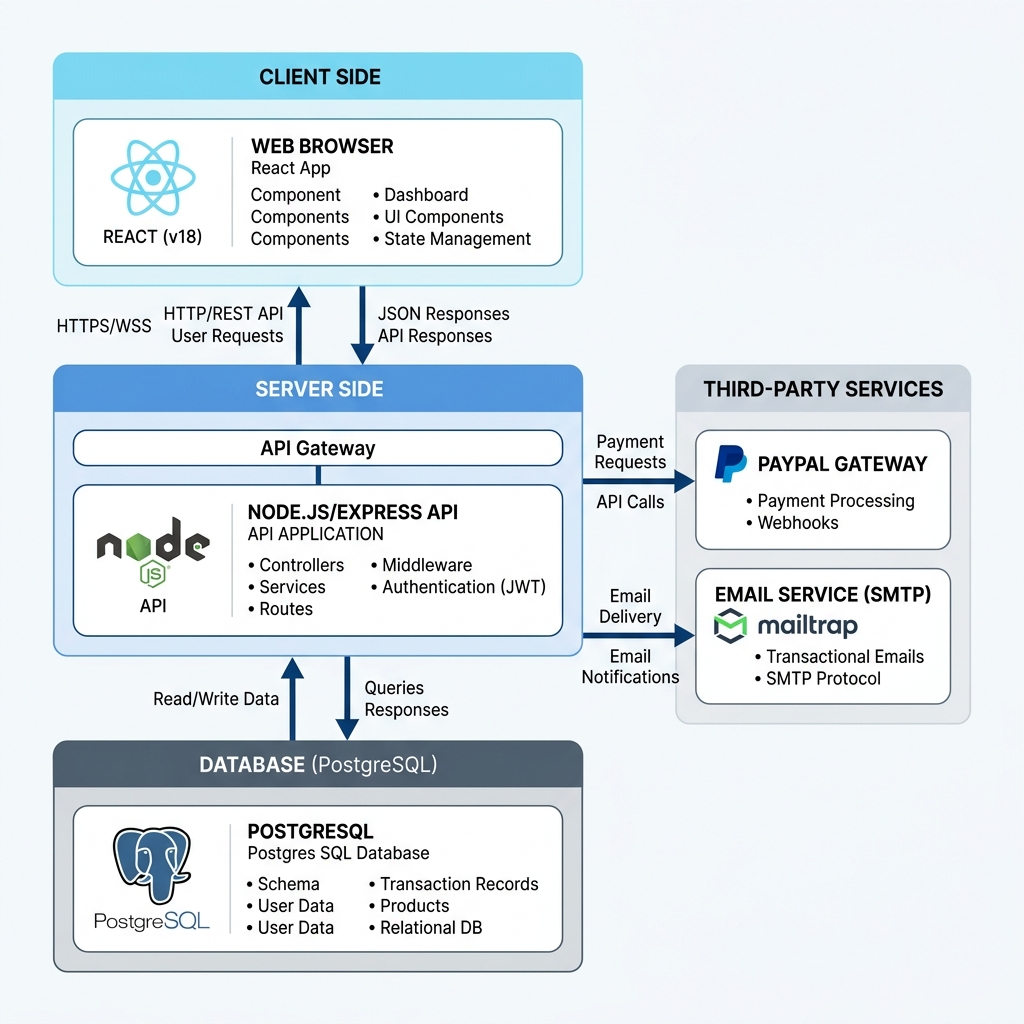
\includegraphics[width=0.85\textwidth]{images/architecture.png}
    \caption{Sơ đồ kiến trúc phần mềm đề xuất}
\end{figure}

Các thành phần cốt lõi được đề xuất bao gồm:

\begin{itemize}
    \item \textbf{Frontend (Lớp hiển thị):} Dự kiến được xây dựng trên nền tảng \textbf{React 19} kết hợp với công cụ build \textbf{Vite}. Giải pháp này cho phép tối ưu hóa tốc độ tải trang và mang lại trải nghiệm mượt mà nhờ \textbf{React Router Dom} (điều hướng) và \textbf{Framer Motion} (hiệu ứng).
    \item \textbf{Backend (Lớp xử lý):} Đề xuất phát triển API RESTful bằng \textbf{Node.js} và framework \textbf{Express 5}. Lớp này sẽ đảm nhiệm việc quản lý phiên làm việc qua \textbf{JWT} và áp dụng các thuật toán mã hóa mạnh mẽ như \textbf{Bcryptjs} để bảo mật dữ liệu người dùng.
    \item \textbf{Cơ sở dữ liệu (Lớp dữ liệu):} Lựa chọn \textbf{PostgreSQL} làm hệ quản trị cơ sở dữ liệu quan hệ chính để đảm bảo tính toàn vẹn của các giao dịch voucher phức tạp.
    \item \textbf{Các giải pháp công nghệ bổ sung:}
    \begin{itemize}
        \item \textbf{Quản lý trạng thái:} Đề xuất sử dụng \textbf{Zustand} để duy trì dữ liệu ứng dụng một cách nhất quán.
        \item \textbf{Tích hợp thanh toán:} Dự kiến tích hợp \textbf{PayPal Sandbox API} để giả lập quy trình thanh toán an toàn.
        \item \textbf{Giao diện:} Lựa chọn \textbf{Tailwind CSS} làm framework thiết kế chủ đạo nhằm đảm bảo tính tương thích đa thiết bị.
        \item \textbf{Hỗ trợ giao tiếp:} Sử dụng \textbf{Nodemailer} cho các tính năng xác thực và gửi mã voucher tự động qua email.
    \end{itemize}
\end{itemize}

\subsection{Phần cứng}
Dự kiến hệ thống sẽ vận hành tốt trên các hạ tầng cơ bản sau:
\begin{itemize}
    \item \textbf{Phía người dùng:} Các thiết bị đầu cuối chạy trình duyệt web hiện đại.
    \item \textbf{Phía máy chủ:} Đề xuất triển khai trên các nền tảng đám mây (Cloud) như \textbf{Railway} hoặc \textbf{Vercel} để tận dụng khả năng tự động hóa và tối ưu chi phí.
\end{itemize}
